\documentclass[12pt,a4paper,UTF8]{ctexart}
\usepackage{graphicx}
\usepackage{amsmath}
\usepackage{amssymb}
\usepackage{subfig}
\usepackage{cite}
\usepackage[ntheorem]{empheq}
\usepackage{enumitem}
\usepackage{fullpage}
\usepackage{cleveref}
\usepackage{cellspace}
\usepackage{listings}
\usepackage{color}
\definecolor{gray}{rgb}{0.5,0.5,0.5}
\definecolor{dkgreen}{rgb}{.068,.578,.068}
\definecolor{dkpurple}{rgb}{.320,.064,.680}

% set Matlab styles
\lstset{
   language=Matlab,
   keywords={break,case,catch,continue,else,elseif,end,for,function,
      global,if,otherwise,persistent,return,switch,try,while},
   basicstyle=\ttfamily,
   keywordstyle=\color{blue}\bfseries,
   commentstyle=\color{dkgreen},
   stringstyle=\color{dkpurple},
   backgroundcolor=\color{white},
   tabsize=4,
   showspaces=false,
   showstringspaces=false
}

\begin{document}
\CJKfamily{zhkai}	


\begin{center}
\textbf{作业二}\\
\textbf{姓名: ~~马宇骁~~~~~~~~ 学号 :~~~PB19151769~~~~~~~~ 日期:~~\today}\\
\end{center}

\begin{center}
\fbox{
\begin{minipage}{40em}
\vspace{5cm}
\hspace{20cm}
\end{minipage}}
\end{center}
\vspace{1cm}

\begin{enumerate}
\item[第一题] \textbf{本题考虑对于定义在$[$-1$,1]$上的一个光滑函数$f(x)$的三次样条插值的使用。下面
所说的误差都是指绝对误差。}

(a)仿照课堂笔记或课本推导出关于额外给定边界点处(即$\textnormal{-}1$和1)三
次样条插值多项式的一次导数值时其在各插值点上的二次导数值应该满足的
线性方程组。请给出推导过程。\\
(b)令三次样条插值多项式在$\textnormal{-}1$和1处的导数为0,用Matlab基于上
一问中的结果使用$n = 2^{4}$个子区间插值一个定义在$[$\textnormal{-}1$,1]$上的函数$f(x) =
sin(4x^{2}) + sin^{2}(4x)$并使用semilogy图通过在2000个等距点上取真实值画出你
构造的三次样条插值的逐点误差。\\
(c)使用不同的n,令$n = 2^{4}, 2^{5}, ..., 2^{10}$重复上一问,取关于不同n的2000个
等距点上的误差的最大值(即横轴是n)。\\
(d)针对周期边界条件,即假设三次样条函数满足$S'($\textnormal{-}1$) = S'(1)$和$S''($\textnormal{-}1$) =S''(1)$,重复完成上面三问中的要求。
\\~

\textbf{\LARGE 解:}

(a)
~ $S_i(x) = a_i + b_i(x - x_i) + c_i(x-x_i)^2 + d_i(x - x_i)^3$

\qquad $S_i(x)' = b_i + 2c_i(x-x_i) + 3d_i(x - x_i)^2$

\qquad $S_i(x)'' = 2c_i + 6d_i(x - x_i)$

令$h_i = x_{i+1}-x_i$,由插值之后的连续性有:

\qquad $a_i + h_i b_i + h_{i}^2 c_i + h_i^3 d_i = y_{i+1} = a_{i+1}$

\qquad $b_i + 2c_ih_i + 3d_ih_i^2 = b_{i+1}$

\qquad $2c_i + 6d_ih_i = 2c_{i+1} = m_{i+1}$

\quad $\Rightarrow m_i + 6d_ih_i = m_{i+1}$

\quad $\Rightarrow h_{i}m_i + 2(h_i + h_{i+1})m_{i+1} + h_{i+1}m_{i+2} = 6(\frac{y_{i+2}-y_{i+1}}{h_{i+1}} - \frac{y_{i+1}-y_i}{h_i})$

\quad 额外给定边界点处: $y_0$与$y_n$已知;
此时将最后一个等式带入插值的点和y的值联立得到方程组解出从1到n-1每一个$m_i$。

$H = 
\begin{pmatrix}
    2(h_0+h_1) & h_1 & 0 & \cdots & \vdots\\
    h_1 & 2(h_1+h_2) & h_2 & 0 & \vdots\\
    0 & \ddots & \ddots & \ddots & 0\\
    \vdots & \cdots & h_{n-1} & 2(h_{n-3}+h_{n-2}) & h_{n-2}\\
    0  & \cdots & \cdots & h_{n-2} & 2(h_{n-2}+h_{n-1}) 
\end{pmatrix},$
$M = 
\begin{pmatrix}
m_1\\
m_2\\
\vdots\\
m_{n-1}
\end{pmatrix},$

$Y = 
\begin{pmatrix}
\frac{y_2-y_1}{h_1}-\frac{y_1-y_0}{h_0}\\
\frac{y_3-y_2}{h_2}-\frac{y_2-y_1}{h_1}\\
\vdots\\
\frac{y_{n}-y_{n-1}}{h_{n-1}}-\frac{y_{n-1}-y_{n-2}}{h_{n-2}}\\
\end{pmatrix}$

\begin{equation}
    HM = 6Y
\end{equation}

此时,带入上式:

\qquad $a_i = y_i$

\qquad $b_i = \frac{y_{i+1} - y_i}{h_i} - \frac{h_i}{2} m_i - \frac{h_i}{6}(m_{i+1}-m_i)$

\qquad $c_i = \frac{m_i}{2}$

\qquad $ d_i = \frac{m_{i+1} - m_i}{6h_i}$

由给边界一阶导数可得
$\Rightarrow m0 = 3*((f(-1+h)-f(-1))/h - h*m_1 - b_0/6)/h;$\\
$a_0 = y_0,b_0 = S'_0(-1),c_0 = m_0/2,d_0 = \frac{m_1-m_0}{6h-0}$
得到n个分段函数;

\textsc{Matlab}程序显示如下:
\begin{lstlisting}[frame=single]
(b)
clear,clc
n = 2^4;
labels = CP(n);
err(labels);

function labels = CP(n)
syms x;
f(x) = sin(4*x^2) + sin(4*x)^2;
%从-1到1,且1阶导为0
%-1和1的边界值已知
h = 2/(n);
Y = zeros(n-1,1);
for k = 1:n-1
    Y(k,1) = (f(-1+(k+1)*h)-f(-1+(k)*h))/h - (f(-1+(k)*h)
    -f(-1+(k-1)*h))/h;
end
H = diag(repmat([4*h],1,n-1))+diag(repmat([h],1,n-2),1)
+diag(repmat([h],1,n-2),-1);
M = H\(6*Y);
m0 = 3*((f(-1+h)-f(-1))/h - h*M(1,1)/6)/h;
mn = 6*((f(1)-f(1-h))/h - h*M(n-1,1)/3)/h;
COE = zeros(n,4);
COE(1,1) = f(-1);
COE(n,1) = f(1-h);
COE(1,2) = 0;
COE(n,2) = 0;
COE(1,3) = m0/2;
COE(n,3) = M(n-1,1)/2;
COE(1,4) = (M(1,1)-m0)/(6*h);
COE(n,4) = (mn-M(n-1,1))/(6*h);
for k = 2:n-1
    COE(k,1) = f(-1+(k-1)*h);
    COE(k,2) = (f(-1+(k)*h)-f(-1+(k-1)*h))/h - h*M(k-1,1)/2 
    - h/6 * (M(k,1)-M(k-1,1));
    COE(k,3) = M(k-1,1)/2;
    COE(k,4) = (M(k,1)-M(k-1,1))/(6*h);
end
d = 2/1999;
labels = zeros(2000,2);
for a = 1:2000
    m = -1+ (a-1)*d;
    labels(a,1) = m;
    k = floor((m+1)/h);
    if k<n
        fx = COE(k+1,1) + COE(k+1,2)*(m+1-h*k) + COE(k+1,3)
        *(m+1-h*k)^2 + COE(k+1,4)*(m+1-h*k)^3;
    else %在1点
        fx = f(1);
    end
    labels(a,2) = abs(sin(4*m^2) + sin(4*m)^2 - fx);
end
end
function err(labels)
semilogy(labels(:,1),labels(:,2),'DisplayName','误差图 ');
% 记录横轴纵轴的数据画图
xlabel('x');
ylabel('误差');
legend
end
\end{lstlisting}
\begin{center}
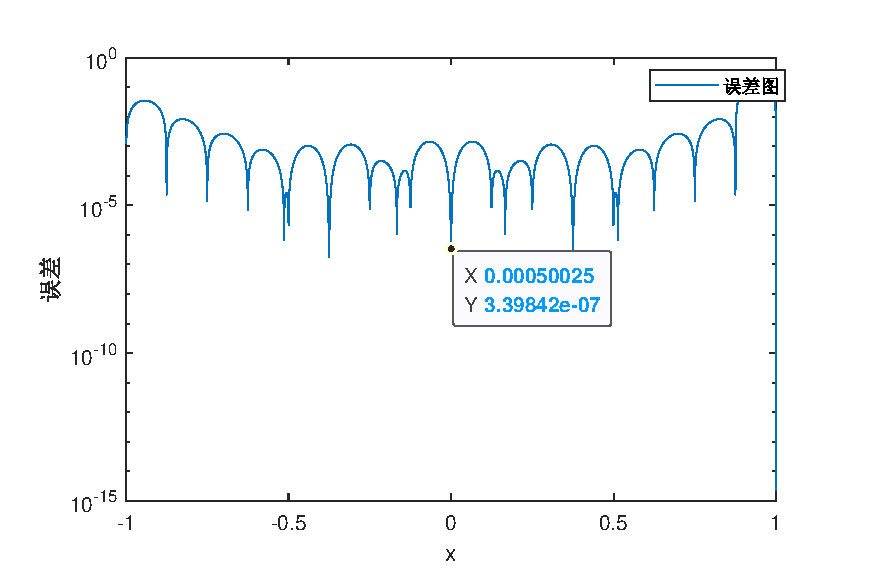
\includegraphics[scale=1]{1b.eps}\\
\end{center}
\textsc{Matlab} (c)新增部分程序显示如下:
\begin{lstlisting}[frame=single]
for k = 4:10
    n = 2^k;
    labels = CP(n);
    MAX(k-3,1)= n;
    [ma,index]=max(labels);
    m = log10(ma(1,2));
    MAX(k-3,2) = m;
end
maxerr(MAX);
function maxerr(labels)
loglog(labels(:,1),labels(:,2),'DisplayName','最大误差
(取log10)');
xlabel('n');
ylabel('log10(误差)');
legend
end
\end{lstlisting}
\begin{center}
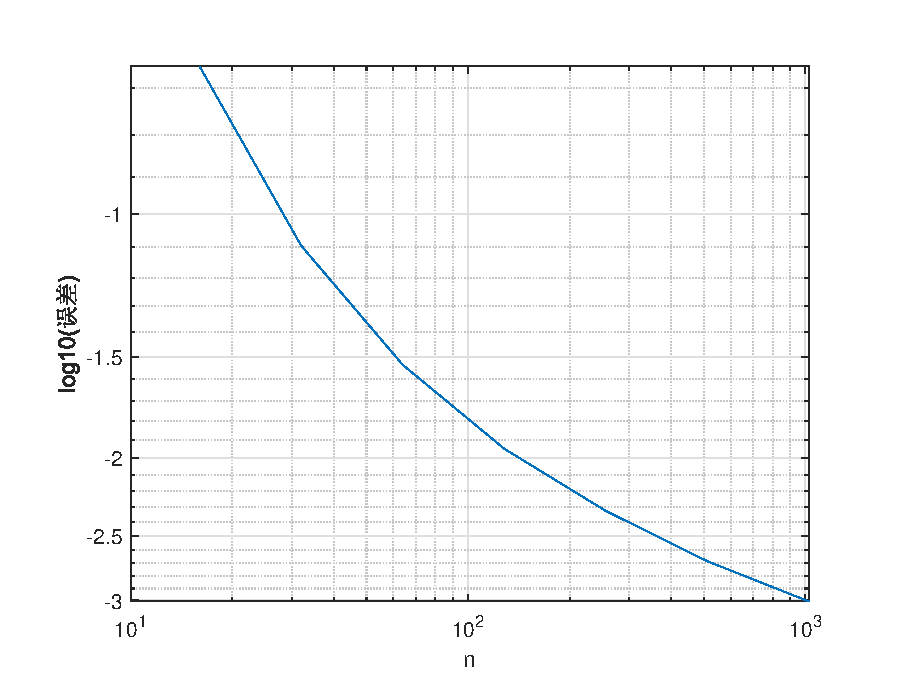
\includegraphics[scale=1]{1c.eps}
\end{center}

(d)

由周期边界条件可得:

\qquad $m_0 = m_n$, $b_0 = b_{n-1}$因此:

$H = 
\begin{pmatrix}
    2(h_0+h_1) & h_1 & 0 & \cdots & h_1\\
    h_2 & 2(h_1+h_2) & h_2 & 0 & \vdots\\
    0 & \ddots & \ddots & \ddots & 0\\
    \vdots & \cdots & h_{n-1} & 2(h_{n-2}+h_{n-1}) & h_{n-1}\\
    h_n  & \cdots & \cdots & h_{n} & 2(h_{n-1}+h_{n}) 
\end{pmatrix},$
$M = 
\begin{pmatrix}
m_1\\
m_2\\
\vdots\\
m_n
\end{pmatrix},$

$Y = 
\begin{pmatrix}
\frac{y_2-y_1}{h_1}-\frac{y_1-y_0}{h_0}\\
\frac{y_3-y_2}{h_2}-\frac{y_2-y_1}{h_1}\\
\vdots\\
\frac{y_{n}-y_{n-1}}{h_{n-1}}-\frac{y_{n-1}-y_{n-2}}{h_{n-2}}\\
\end{pmatrix}$

\begin{equation}
    HM = 6Y
\end{equation}

\textsc{Matlab}程序显示如下:
\begin{lstlisting}[frame=single]
clear,clc
n = 2^4;
labels = CP(n);
err(labels);
for k = 4:10
    n = 2^k;
    labels = CP(n);
    MAX(k-3,1)= n;
    [ma,index]=max(labels);
    m = log10(ma(1,2));
    MAX(k-3,2) = m;
end
maxerr(MAX);

function labels = CP(n)
syms x;
f(x) = sin(4*x^2) + sin(4*x)^2;
%从-1到1,且1阶导为0
%-1和1的边界值连续
h = 2/(n);
Y = zeros(n,1);
for l = 1:n
    k = l+1;
    Y(l,1) = (f(-1+k*h)-f(-1+(k-1)*h))/h 
    - (f(-1+(k-1)*h)-f(-1+(k-2)*h))/h;
end
H = diag(repmat([4*h],1,n))+diag(repmat([h],1,n-1),1)
+diag(repmat([h],1,n-1),-1);
H(1,n) = h;
H(n,1) = h;
M = H\(6*Y);
M = [M(n,1);M];
COE = zeros(n,4);
for k = 1:n
    COE(k,1) = f(-1+(k-1)*h);
    COE(k,2) = (f(-1+(k)*h)-f(-1+(k-1)*h))/h - h*M(k,1)/2 
    - h/6 * (M(k+1,1)-M(k,1));
    COE(k,3) = M(k,1)/2;
    COE(k,4) = (M(k+1,1)-M(k,1))/(6*h);
end
d = 2/1999;
labels = zeros(2000,2);
for a = 1:2000
    m = -1+ (a-1)*d;
    labels(a,1) = m;
    k = floor((m+1)/h);
    if k<n
        fx = COE(k+1,1) + COE(k+1,2)*(m+1-h*k) + COE(k+1,3)
        *(m+1-h*k)^2 + COE(k+1,4)*(m+1-h*k)^3;
    else %在1点
        fx = f(1);
    end
    labels(a,2) = abs(sin(4*m^2) + sin(4*m)^2 - fx);
end
end

function maxerr(labels)
semilogy(labels(:,1),labels(:,2),'DisplayName',
'最大误差(取log10) ');
% 记录横轴纵轴的数据画图
xlabel('n');
ylabel('log10(误差)');
legend
end
function err(labels)
loglog(labels(:,1),labels(:,2),'DisplayName','误差图 ');
% 记录横轴纵轴的数据画图
xlabel('x');
ylabel('误差');
legend
end
\end{lstlisting}
\begin{center}
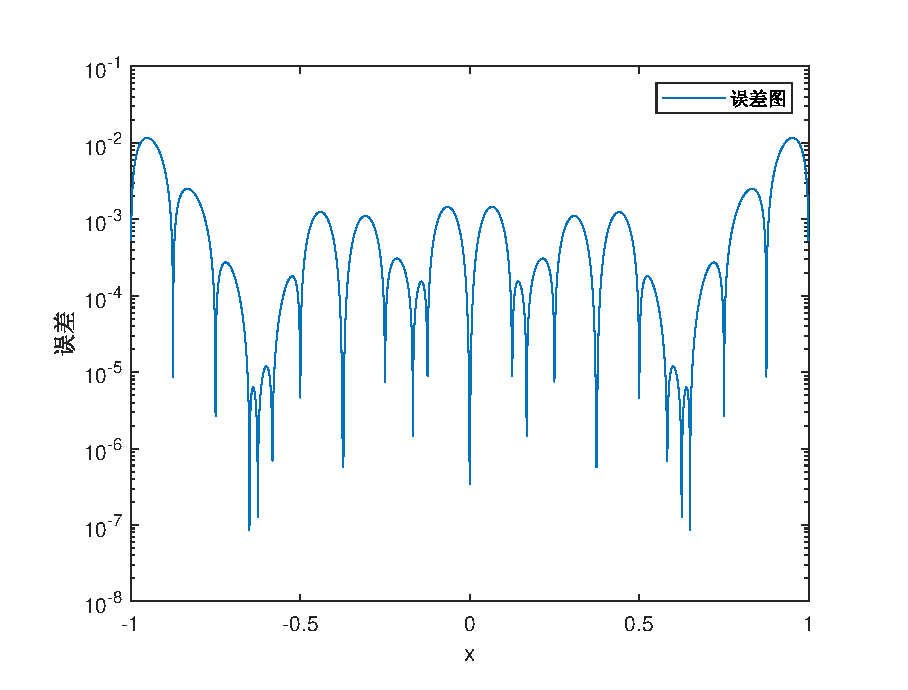
\includegraphics[scale=1]{1db.eps}\\
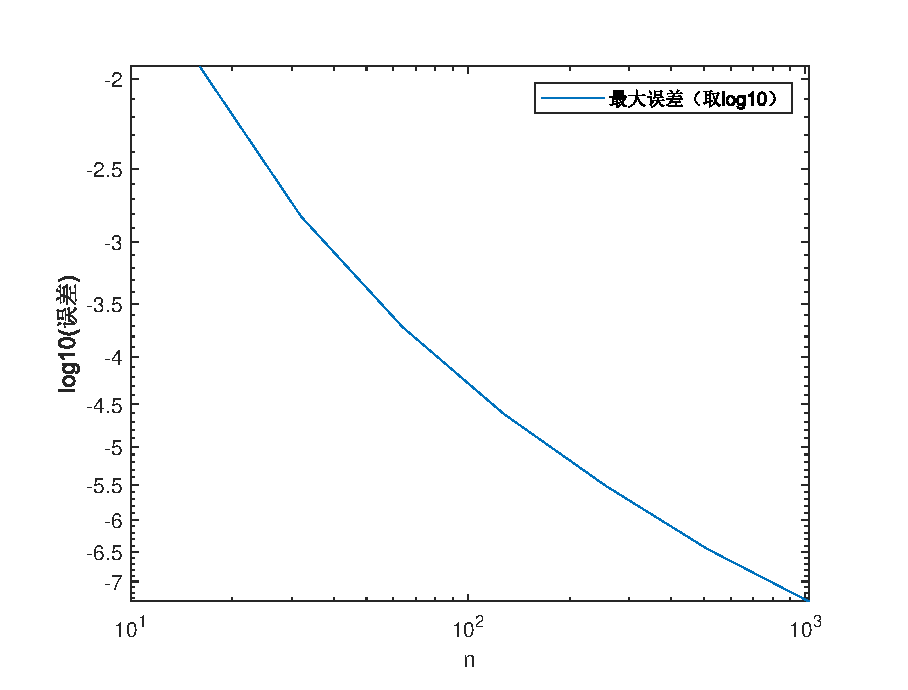
\includegraphics[scale=1]{1dc.eps}\\
\end{center}



\item[第二题] \textbf{本题深入讨论Newton插值公式的性质。}
 
(a)对于一个光滑函数$f(x)$,证明若$\left\{i_0, i_1, ..., i_k\right\}$是$\left\{0, 1, ..., k\right\}$的任意一
个排列,则$$f[x_0, x_1, ..., x_k] = f[x_{i0}, x_{i1}, ..., x_{ik}]$$\\
(b)课堂上我们提到了Chebyshev点$$x_j = cos(j\pi/n)~~~~j = 0, 1, ..., n$$
以及使用Chebyshev点可以有效地克服Runge现象。写一个Matlab程序,令
$n = 2^{2}, 2^{3}, 2^{4}, ..., 2^{7}$,按照从右到左的顺序(即j从小到大的顺序)使用对应
的$n + 1$个
Chebyshev点对定义在$[$\textnormal{-}1$,1]$上的Runge函数$$f(x) = \frac{1}{1 + 25x^{2}}$$
进行插值,并取2000个等距点上的误差的最大值,用semilogy图描述插值区
间上最大误差值随n变化的情况(即横轴是n)。\\
(c)重复上一问,但使用随机数种子rng(22)和randperm函数来随机计算
差商时插值点的使用顺序,取关于不同n的2000个等距点上的误差的最大值,
用semilogy图描述插值区间上最大误差值随n变化的情况(即横轴是n)。\\
(d)试着解释上面两小问中你观察到的不同现象产生的原因。注:此问
答不出来也无妨。
\\~

\textbf{\LARGE 解:}

(a) 由定义可知:

\qquad $f[x_0,x_1] = \frac{f(x_1)-f(x_0)}{x_1 - x_0}$

\qquad $f[x_0,x_1,x_2] = \frac{f[x_1,x_2]-f[x_0,x_1]}{x_2 - x_0}$

\qquad \qquad $\Rightarrow \qquad = \frac{f(x_0)}{(x_0-x_1)(x_0-x_2)} + \frac{f(x_1)}{(x_1-x_0)(x_1-x_2)} + \frac{f(x_2)}{(x_2-x_0)(x_2-x_1)}$

\qquad \qquad \vdots

\qquad $f[x_0,x_1,...,x_k] = \frac{f[x_1,x_2,...,x_k]-f[x_0,x_1,...,x_{k-1}]}{x_k - x_0}$

\qquad \qquad $\Rightarrow \qquad = \frac{f[x_2,x_3,...,x_k]-f[x_1,x_2,...,x_{k_1}]}{(x_k-x_0)(x_k-x_1)} - \frac{f[x_1,x_2,...,x_{k-1}]-f[x_0,x_1,...,x_{k_2}]}{(x_k-x_0)(x_{k-1}-x_0)}$

\qquad \qquad $\Rightarrow \qquad \vdots$

\qquad \qquad $\Rightarrow \qquad = \sum_{i = 0}^{k} \frac{f(x_i)}{(x_i-x_0)\cdots(x_i-x_{i-1})(x_i-x{i+1})\cdots(x_i-x_k)}$

同理:

\qquad $f[x_{i0},x_{i1},...,x_{ik}] = \sum_{j = 0}^{k} \frac{f(x_{ji})}{(x_{ji}-x_{0i})\cdots(x_{ji}-x_{(j-1)i})(x_{ji}-x{(j+1)i})\cdots(x_{ji}-x_{ki})}$\\

再由$\left\{i_0, i_1, ..., i_k\right\}$是$\left\{0, 1, ..., k\right\}$的任意一个排列,由求和的遍历性:

\vspace*{-0.5cm}
\qquad $$f[x_0, x_1, ..., x_k] = f[x_{i0}, x_{i1}, ..., x_{ik}]$$\\

\textsc{Matlab}程序显示如下:
\begin{lstlisting}[frame=single]
(b)
clear,clc

for k = 2:7
    maxr = CHENew(2^k);
    labels(k-1,1) = 2^k;
    labels(k-1,2) = maxr;
end
err(labels);

function r = CHENew(n)
syms x;
f(x) = 1/(1+25*x^2);
X(1) = cos(0);
Y(1) = f(X(1));
for i = 2:n+1
    X(i) = cos((i-1)*pi/n);
    Y(i) = f(X(i));
end
F=zeros(n+1,n+1);
for k=1:n+1      
    F(k,1)=Y(k);
end
for k=2:n+1 
    for l=k:n+1
        F(l,k)=(F(l,k-1)-F(l-1,k-1))/(X(l)-X(l+1-k));  
    end
end
m = 1999;
for k = 1:m+1
    k
    labels(k,1) = -1+(k-1)/m;
    g = F(1,1);
    for j = 2:n+1
        P = 1;
        for l = 1:j-1
            P = P * (labels(k,1) - X(l));
        end
        g = F(j,j) * P + g;
    end
    labels(k,2) = abs(g - f(labels(k,1)));
end
r = max(labels(:,2));
end

function err(labels)
semilogy(labels(:,1),labels(:,2),'DisplayName','误差图 ');
% 记录横轴纵轴的数据画图
xlabel('n');
ylabel('最大误差');
legend
end
\end{lstlisting}
\begin{center}
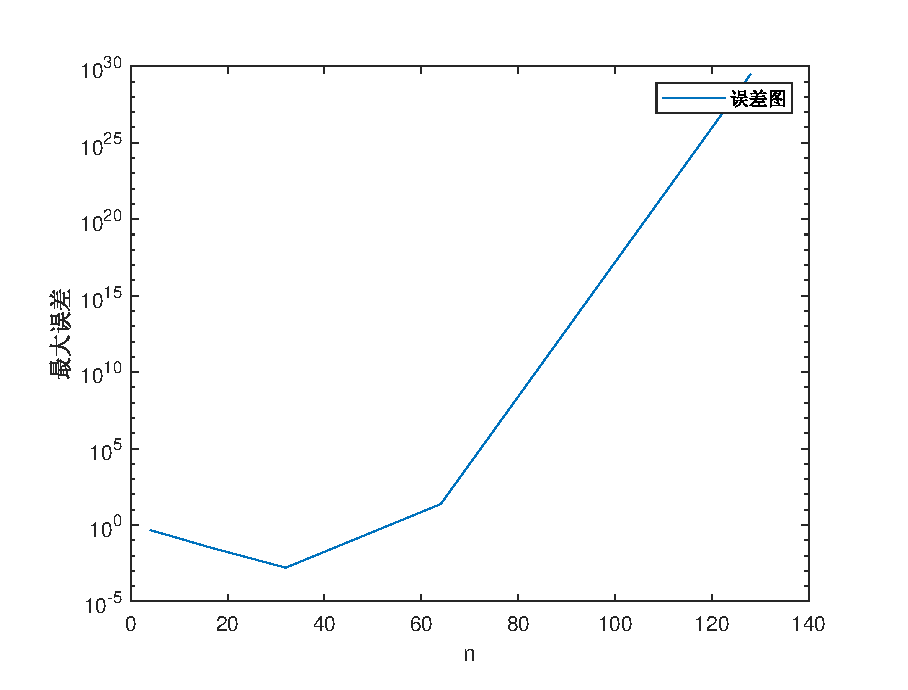
\includegraphics[scale=1]{2b.eps}\\
\end{center}

\textsc{Matlab}程序显示如下:(省略重复函数)
\begin{lstlisting}[frame=single]
(c)
clear,clc

for k = 2:7
    ran = rand(2^k);
    maxr = CHENew(2^k,ran);
    labels(k-1,1) = 2^k;
    labels(k-1,2) = maxr;
end
err(labels);

function r = CHENew(n,ran)
syms x;
f(x) = 1/(1+25*x.^2);
X(1) = ran(1,1);
Y(1) = f(X(1));
for i = 2:n+1
    X(i) = ran(i,1);
    Y(i) = f(X(i));
end
F=zeros(n+1,n+1);
for k=1:n+1      
    F(k,1)=Y(k);
end
for k=2:n+1 
    for l=k:n+1
        F(l,k)=(F(l,k-1)-F(l-1,k-1))/(X(l)-X(l+1-k));  
    end
end
m = 1999;
for k = 1:m+1
    k
    labels(k,1) = -1+(k-1)/m;
    g = F(1,1);
    for j = 2:n+1
        P = 1;
        for l = 1:j-1
            P = P * (labels(k,1) - X(l));
        end
        g = F(j,j) * P + g;
    end
    labels(k,2) = abs(g - f(labels(k,1)));
end
r = max(labels(:,2));
end

function ran = rand(n)
    rng(22);
    r = randperm(n+1,n+1);
    for k = 1 : n + 1
        ran(k,1) = cos((r(k) - 1) * pi / n);
    end
end
end
\end{lstlisting}
\begin{center}
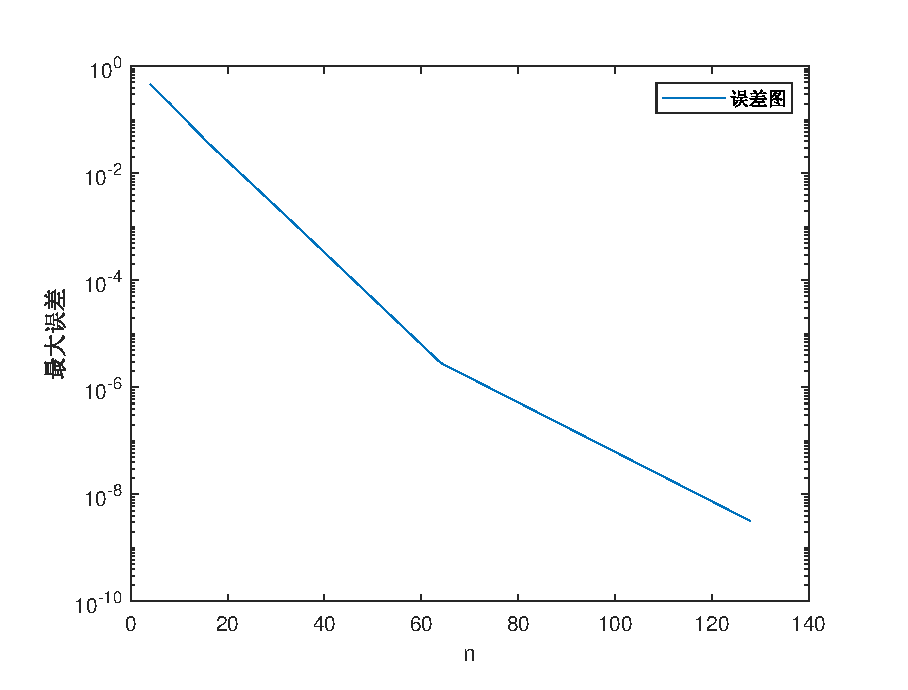
\includegraphics[scale=1]{2c.eps}\\
\end{center}

(d) 

MATLAB自身在计算三角函数的时候就采取近似处理,使得切比雪夫点的计算误差一直存在且约偏离误差越大,
于是造成在第b问j等距计算切比雪夫点插值的时候的精确度到一定阶段随着点插入曾多精度不能保证,反而下降。


\item[第三题] \textbf{本题用于讨论周期函数的Lagrange插值方法。对于周期函数而言,多项式不再是
最有效的基函数,而等距插值点也不再会出现Runge现象。逼近周期函数的基函
数通常选用三角函数或者复指数。同时注意对于周期函数而言,插值点数量和子
区间个数相等。
}

(a)在$[$\textnormal{-}1$,1]$上关于周期函数的基于等间距插值点$x_j = \frac{j}{n},j = 0,1, ...,
n~$\textnormal{-} 1$ $的Lagrange插值基函数为
$$\ell_k(x) = \begin{cases}
\frac{(-1)^{k}}{n}sin(n\pi x)csc(\pi(x - x_k))~~~~&若n为奇数\\
\frac{(-1)^{k}}{n}sin(n\pi x)cot(\pi(x - x_k))~~~~&若n为偶数\\
\end{cases}$$
证明对于n分别为奇数和偶数的情况下
$$\ell_k(x_j) = \begin{cases}
1~~~~&k = j\\
0~~~~&k \neq j\\
\end{cases}$$\\
(b)用上述对应于n为偶数的Lagrange基函数构造Lagrange插值多项式,
并用$n = 2^{6}$个点对周期函数$f(x) = sin(2\pi x)e^{cos(2\pi x)}$
在$[$\textnormal{-}1$,1]$上进行插值。取1000个
等距点上的误差,用semilogy图描述插值区间上误差值随x变化的情况(即
横轴是x)。
\\ 

\textbf{解:}

(a)由题得:$j = 0,1,2,...,n-1, x_j = j/n$\\
\\~
n为奇数时:
\qquad $l_k(x_j) = \frac{(-1)^k}{n}~sin(\pi j)~\frac{1}{sin(\pi(x_j - x_k))}$

显然,若$j \neq k, sin(\pi j)=0, 0 < |x_j - x_k| < 1, \frac{1}{sin(\pi(x_j - x_k))} \neq 0$

\quad $\Rightarrow l_k(x_j) = 0$

k = j 时,$sin(\pi(x_j - x_k) = 0, sin(\pi(x_j - x_k)) = 0$

\qquad $\lim\limits_{j \to k} sin(n\pi x_j)~\frac{1}{sin(\pi(x_j - x_k))} = (-1)^k n$

\quad $\Rightarrow l_k(x_j) = 1$\\
n为偶数时:

\qquad $l_k(x_j) = \frac{(-1)^k}{n}~sin(\pi j)~\frac{cos(\pi(x_j - x_k)}{sin(\pi(x_j - x_k))}$

显然,若$j \neq k, sin(\pi j)=0, 0 < |x_j - x_k| < 1, \frac{cos(\pi(x_j - x_k)}{sin(\pi(x_j - x_k))} \neq 0$

\quad $\Rightarrow l_k(x_j) = 0$

k = j 时,$sin(\pi(x_j - x_k) = 0, sin(\pi(x_j - x_k)) = 0$

\qquad $\lim\limits_{j \to k} sin(n\pi x_j)~\frac{cos(\pi(x_j - x_k))}{sin(\pi(x_j - x_k))} = (-1)^k n$

\quad $\Rightarrow l_k(x_j) = 1$

\textsc{Matlab}程序显示如下:
\begin{lstlisting}[frame=single]
clear,clc

syms x;
n = 2^6;
f(x) = sin(2*pi*x)*exp(cos(2*pi*x));
for k = 1:n
    Y(k) = f((k-1)/n);
end
syms y;
for j = 0 : n - 1 
    L(j+1) = ((-1)^j)/n * sin(n*pi*y) * cot(pi*(y-j/n));
end
P(y) = Y(1) * L(1);
for k = 2 : n
    P(y) = P(y) + Y(k) * L(k);
end
m = 999;
for ka = 1:m+1
    k = ka-1
    labels(ka,1) = k/m;
    labels(ka,2) = abs(P(k/m)-f(k/m));
end

er(labels);

function er(labels)
semilogy(labels(:,1),labels(:,2),'DisplayName',
'Lagrange误差图 ');
% 记录横轴纵轴的数据画图
xlabel('x');
ylabel('误差');
legend
end
\end{lstlisting}
\begin{center}
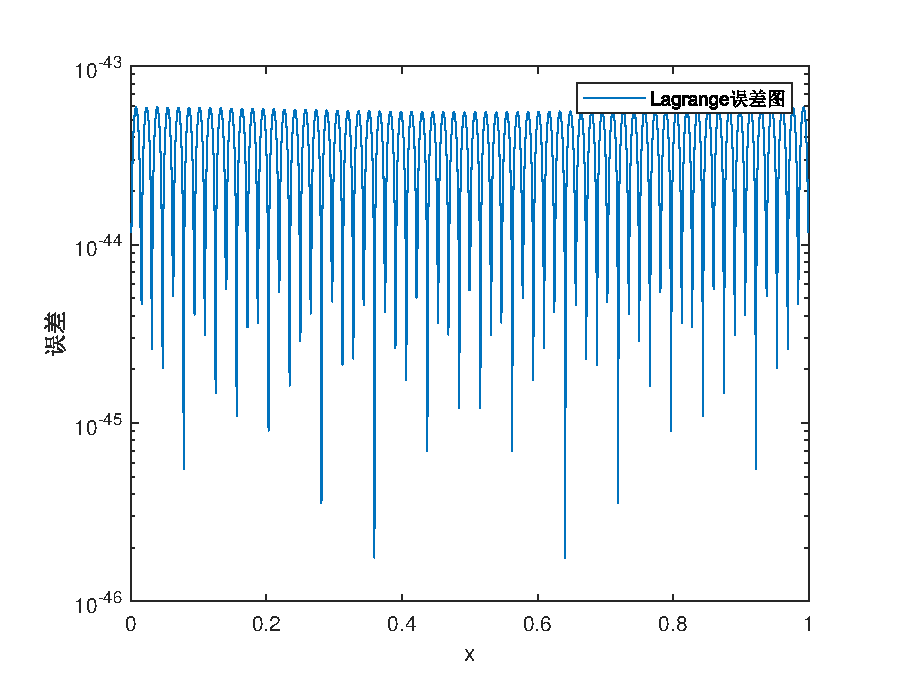
\includegraphics[scale=1]{3b.eps}\\
\end{center}
    
\item[第四题] \textbf{写程序完成课本59页第7题,并计算出你的拟合函数对比所给数据点的
误差的2-范数。}
\\ 
\textsc{Matlab}程序显示如下:
\begin{lstlisting}[frame=single]
    clear,clc
X = [2.1;2.5;2.8;3.2];
Y = [0.6087;0.6849;0.7368;0.8111];
syms a;
syms b;
for k = 1:4
    Y1(k) = X(k)/(a + b*X(k));
end
L(a,b) = (Y(1) - Y1(1))^2;
for k = 2:4
    L(a,b) = L(a,b) + (Y(k) - Y1(k))^2;
end
La(a,b) = diff((L(a,b)),a);
Lb(a,b) = diff((L(a,b)),b);
eqns = [La(a,b)==0,Lb(a,b)==0];
[a0,b0] = solve(eqns,[a,b]);
a0 = vpa(a0);
b0 = vpa(b0);
a0 = min(a0);
b0 = min(b0);
syms x;
f(x) = x/(a0 + b0 * x);
for k = 1:4
    Y2(k) = abs(f(X(k))-Y(k)); %误差
end
norm2 = norm(Y2,2)
\end{lstlisting}
\begin{center}
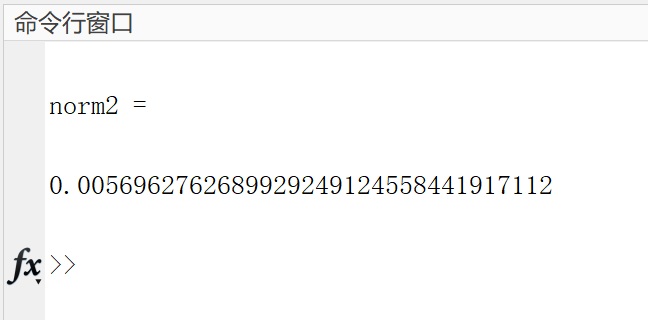
\includegraphics[scale=0.6]{4.png}\\
\end{center}
\end{enumerate}
\end{document}
